\section{Prepoznavanje naredbi i aktivacija zadatka}

Ukoliko se mreža aktivira dovoljno često, za očekivati je da će najvjerojatniji izlaz iz 
neuronske mreže u slučaju izgovorene naredbe biti upravo kategorija koja predstavlja tu naredbu. 
Štoviše, naredba bi trebalča biti prepoznata u više uzastopnih iteracija aktiviranja mreže.
Međutim, ponašanje sustava u tom slučaju neće biti onakvo kakvo bi trebalo, a to je da se
određeni posao (zadatak) aktivira isključivo jednom za jednom izgovorenu naredbu. 
Još jedna stvar na koju treba pripaziti je slučajno aktiviranje nekog posla jer zbog
nesavršenosti mreže se može dogoditi da vjerojatnosni izlaz ukazuje na prepoznavanje neke
naredbe. Međutim, u takvim situacijama se očekuje možda jedna ili dvije takve situacije zaredom,
a ne više njih. Zbog svega navedenog, potrebno je na neki način obraditi tok vjerojatnosnih
izlaza iz neuronske mreže. Kao najbolji način za pokrivanje svih problema pokazalo se 
uprosjećivanje vjerojatnosti pojedinih kategorija. 

Na slici \ref{pic:uml} prikazan je UML dijagram implementiranog podsustava. Glavni dio posla
obavlja se unutar razreda \texttt{CommandRecognizer} koji je zadužen za čuvanje informacije
o vjerojatnostima za pojedinu kategoriju naredbi u zadnjih nekoliko iteracija, računanje
prosječne vjerojatnosti te aktiviranje obavljanja konkretnog posla koji je povezan s govornom
naredbom. Također, potreban je period vremena u kojem se nakon aktivacije određenog
posla, ne može opet aktivirati isti. Parametri koji su podesivi i potrebno ih je odrediti 
eksperimentalno su broj vrijednosti nad kojima se računa prosjek (koliko se posljednjih
vjerojatnosti čuva), razina iznad koje se naredba smatra prepoznatom i pokreće prikladni zadatak
te vrijeme perioda u kojem nije moguće opet aktivirati naredbu. 

\begin{figure}[htb]
    \centering
    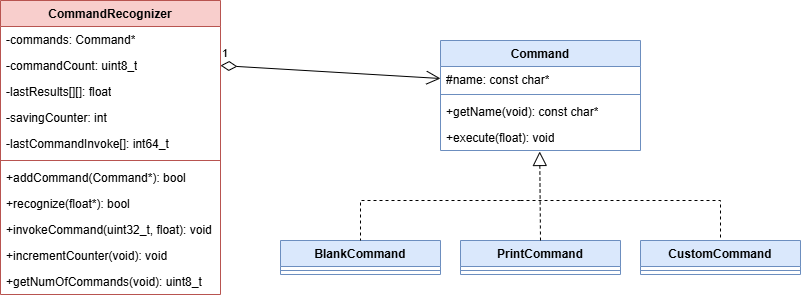
\includegraphics[width=0.8\linewidth]{Chapters/struktura_sustava/prepoznavanje_naredbi/commands.png} 
    \caption{Podsustav za prepoznavanje naredbi i aktivaciju zadataka\cite{flowchart}}
    \label{pic:uml}
\end{figure}

Razred \texttt{CommandRecognizer} sadrži listu pokazivača na objekte čiji razredi implementiraju 
sučelje \texttt{Command}. \texttt{Command} predstavlja sučelje (apstraktni razred) što znači da
nije moguće konstruirati objekt tog razreda, nego da je potrebno naslijediti razredom koji 
implementira apstraktnu metodu \texttt{virtual void execute(float probability)}. Ta 
metoda je zadužena za obavljanje konkretnog zadatka. Ovakav strukturni
obrazac daje mogućnost vrlo lakog implementiranja novih vrsta zadataka (sve što je potrebno je 
napraviti novi razred koji implementira sučelje \texttt{Command}). Trenutno su implementirane
dvije vrste naredbi (zadataka): \texttt{BlankCommand} koja ne radi ništa (koristi se za kategorije
"pozadina" i "nepoznato") i \texttt{PrintCommand} koja ispisuje ime naredbe i prosječnu 
vjerojatnost pojavljivanja naredbe. Jednom konstruirani objekt naredbe potrebo je dodati 
u objekt klase CommandRecognizer metodom \texttt{bool addCommand(Command* command)} 
kako bi on bio svjestan postojanja te naredbe (broj izlaza iz neuronske mreže mora odgovarati 
broju dodatnih naredbi ovim putenm). Svaka konkretna implementacija metode 
\texttt{virtual void execute(float probability)} ne smije trajati predugo jer će unijeti 
kašnjenje u cjelokupni sustav. Ideja je da takva naredba samo pokrene duži posao za koji će onda
biti zadužen neki drugi sustav.